\documentclass[11pt]{article}\usepackage[]{graphicx}\usepackage[table]{xcolor}
% maxwidth is the original width if it is less than linewidth
% otherwise use linewidth (to make sure the graphics do not exceed the margin)
\makeatletter
\def\maxwidth{ %
  \ifdim\Gin@nat@width>\linewidth
    \linewidth
  \else
    \Gin@nat@width
  \fi
}
\makeatother

\definecolor{fgcolor}{rgb}{0.345, 0.345, 0.345}
\newcommand{\hlnum}[1]{\textcolor[rgb]{0.686,0.059,0.569}{#1}}%
\newcommand{\hlstr}[1]{\textcolor[rgb]{0.192,0.494,0.8}{#1}}%
\newcommand{\hlcom}[1]{\textcolor[rgb]{0.678,0.584,0.686}{\textit{#1}}}%
\newcommand{\hlopt}[1]{\textcolor[rgb]{0,0,0}{#1}}%
\newcommand{\hlstd}[1]{\textcolor[rgb]{0.345,0.345,0.345}{#1}}%
\newcommand{\hlkwa}[1]{\textcolor[rgb]{0.161,0.373,0.58}{\textbf{#1}}}%
\newcommand{\hlkwb}[1]{\textcolor[rgb]{0.69,0.353,0.396}{#1}}%
\newcommand{\hlkwc}[1]{\textcolor[rgb]{0.333,0.667,0.333}{#1}}%
\newcommand{\hlkwd}[1]{\textcolor[rgb]{0.737,0.353,0.396}{\textbf{#1}}}%
\let\hlipl\hlkwb

\usepackage{framed}
\makeatletter
\newenvironment{kframe}{%
 \def\at@end@of@kframe{}%
 \ifinner\ifhmode%
  \def\at@end@of@kframe{\end{minipage}}%
  \begin{minipage}{\columnwidth}%
 \fi\fi%
 \def\FrameCommand##1{\hskip\@totalleftmargin \hskip-\fboxsep
 \colorbox{shadecolor}{##1}\hskip-\fboxsep
     % There is no \\@totalrightmargin, so:
     \hskip-\linewidth \hskip-\@totalleftmargin \hskip\columnwidth}%
 \MakeFramed {\advance\hsize-\width
   \@totalleftmargin\z@ \linewidth\hsize
   \@setminipage}}%
 {\par\unskip\endMakeFramed%
 \at@end@of@kframe}
\makeatother

\definecolor{shadecolor}{rgb}{.97, .97, .97}
\definecolor{messagecolor}{rgb}{0, 0, 0}
\definecolor{warningcolor}{rgb}{1, 0, 1}
\definecolor{errorcolor}{rgb}{1, 0, 0}
\newenvironment{knitrout}{}{} % an empty environment to be redefined in TeX

\usepackage{alltt}
%\usepackage[showframe]{geometry}
\usepackage[table]{xcolor}
\usepackage{caption}
\usepackage{lscape,verbatim,mathrsfs}
\usepackage{graphics,amsmath,pstricks}
\usepackage{amssymb,enumerate}
\usepackage{amsbsy,amsmath,amsthm,amsfonts, amssymb}
\usepackage{graphicx, rotate, array}
\usepackage{geometry,multirow}
\usepackage{color,soul}
\usepackage{float}
%\usepackage{hyperref}
\usepackage[authoryear,round]{natbib}
%\renewcommand{\baselinestretch}{1.9}
\usepackage{tcolorbox}
\renewcommand{\familydefault}{cmss}
\textwidth=6.65in \textheight=9.7in
\parskip=.025in
\parindent=0in
\oddsidemargin=-0.1in \evensidemargin=-.1in \headheight=-.6in
\footskip=0.5in \DeclareMathOperator*{\argmax}{argmax}
\DeclareMathOperator*{\argmin}{argmin}
\IfFileExists{upquote.sty}{\usepackage{upquote}}{}
\begin{document}
%\SweaveOpts{concordance=TRUE}










\begin{knitrout}
\definecolor{shadecolor}{rgb}{0.969, 0.969, 0.969}\color{fgcolor}
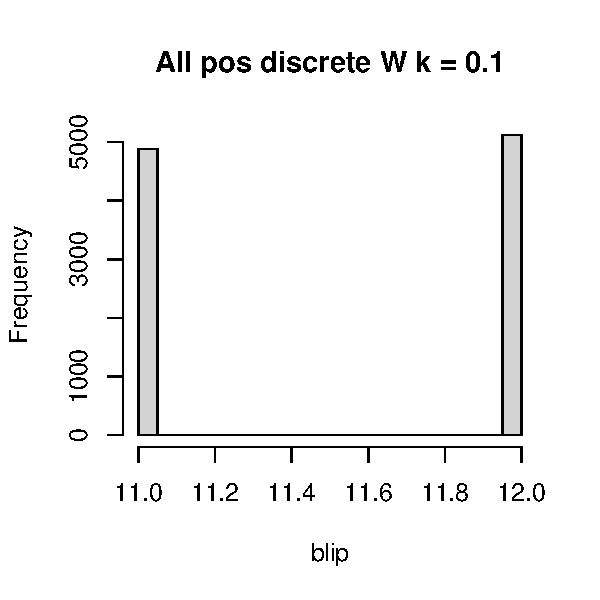
\includegraphics[width=\maxwidth]{figure/unnamed-chunk-4-1} 
\begin{kframe}\begin{verbatim}
##                         desc    bias_psi bias_cont_EY0 bias_cont_EY1
## 1 All pos discrete W k = 0.1 0.001288696  -0.004810103  -0.004810103
##       var_psi var_cont_EY0 var_cont_EY1 cov_psi cov_cont_EY0 cov_cont_EY1
## 1 0.001967655 8.605428e-05   0.00347095    0.95        0.911        0.957
##   cov_da_psi cov_da_cont_EY0 cov_da_cont_EY1 regret tauP0vtauPn
## 1      0.962           0.949            0.96      0 0.001542919
\end{verbatim}
\end{kframe}
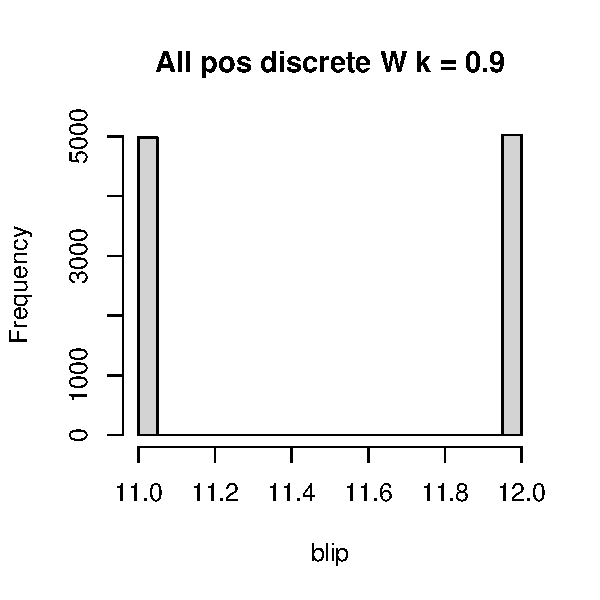
\includegraphics[width=\maxwidth]{figure/unnamed-chunk-4-2} 
\begin{kframe}\begin{verbatim}
##                         desc    bias_psi bias_cont_EY0 bias_cont_EY1
## 1 All pos discrete W k = 0.9 0.004662456   0.004545666   0.004545666
##       var_psi var_cont_EY0 var_cont_EY1 cov_psi cov_cont_EY0 cov_cont_EY1
## 1 0.002710646  0.003493437 8.307476e-05   0.945        0.956        0.926
##   cov_da_psi cov_da_cont_EY0 cov_da_cont_EY1 regret tauP0vtauPn
## 1      0.982           0.955           0.947      0 0.001098835
\end{verbatim}
\end{kframe}
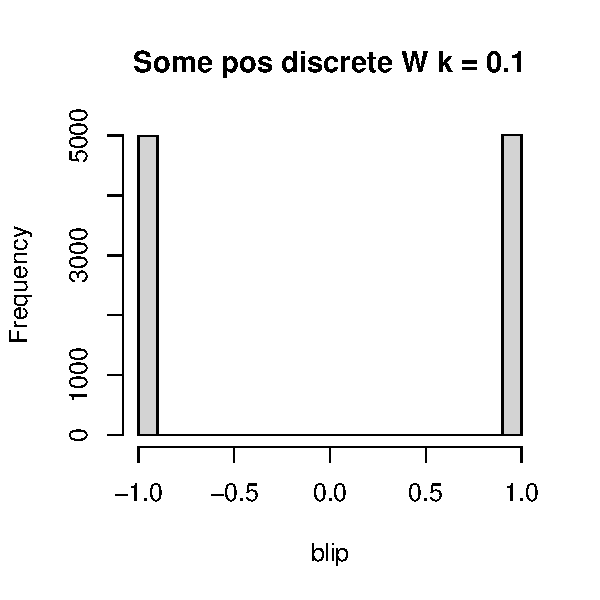
\includegraphics[width=\maxwidth]{figure/unnamed-chunk-4-3} 
\begin{kframe}\begin{verbatim}
##                          desc    bias_psi bias_cont_EY0 bias_cont_EY1
## 1 Some pos discrete W k = 0.1 0.006094873   0.009036945   0.009036945
##       var_psi var_cont_EY0 var_cont_EY1 cov_psi cov_cont_EY0 cov_cont_EY1
## 1 0.002012113 8.350379e-05  0.004515191   0.936        0.832        0.939
##   cov_da_psi cov_da_cont_EY0 cov_da_cont_EY1 regret tauP0vtauPn
## 1       0.96            0.95           0.979      0 0.001098835
\end{verbatim}
\end{kframe}
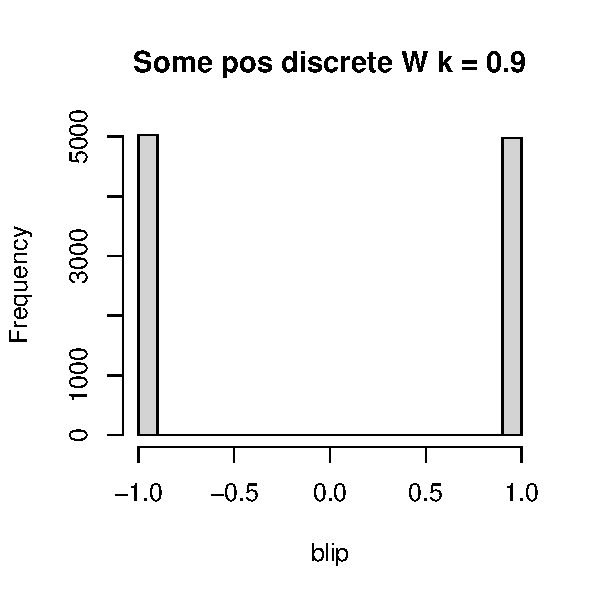
\includegraphics[width=\maxwidth]{figure/unnamed-chunk-4-4} 
\begin{kframe}\begin{verbatim}
##                          desc     bias_psi bias_cont_EY0 bias_cont_EY1
## 1 Some pos discrete W k = 0.9 -0.001149394  -0.002007521  -0.002007521
##      var_psi var_cont_EY0 var_cont_EY1 cov_psi cov_cont_EY0 cov_cont_EY1
## 1 0.00218299  0.002325896  0.002416829   0.935        0.951        0.947
##   cov_da_psi cov_da_cont_EY0 cov_da_cont_EY1 regret tauP0vtauPn
## 1      0.933           0.956            0.96      0           0
\end{verbatim}
\end{kframe}
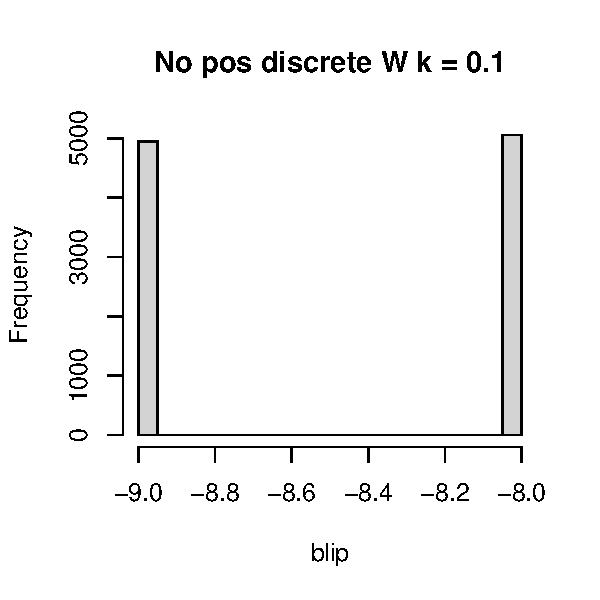
\includegraphics[width=\maxwidth]{figure/unnamed-chunk-4-5} 
\begin{kframe}\begin{verbatim}
##                        desc     bias_psi bias_cont_EY0 bias_cont_EY1
## 1 No pos discrete W k = 0.1 -0.002043563   0.001730347   0.001730347
##       var_psi var_cont_EY0 var_cont_EY1 cov_psi cov_cont_EY0 cov_cont_EY1
## 1 0.002205179 6.224954e-32  0.004206451   0.945            0        0.955
##   cov_da_psi cov_da_cont_EY0 cov_da_cont_EY1 regret tauP0vtauPn
## 1      0.961           0.206           0.957      0           0
\end{verbatim}
\end{kframe}
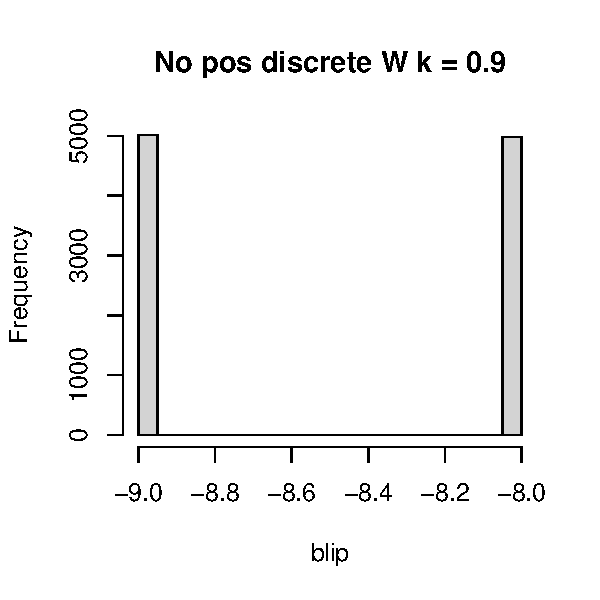
\includegraphics[width=\maxwidth]{figure/unnamed-chunk-4-6} 
\begin{kframe}\begin{verbatim}
##                        desc     bias_psi bias_cont_EY0 bias_cont_EY1
## 1 No pos discrete W k = 0.9 0.0006449771  0.0002538227  0.0002538227
##       var_psi var_cont_EY0 var_cont_EY1 cov_psi cov_cont_EY0 cov_cont_EY1
## 1 0.002205179 6.224954e-32  0.004206451   0.948            0        0.954
##   cov_da_psi cov_da_cont_EY0 cov_da_cont_EY1 regret tauP0vtauPn
## 1      0.961           0.206           0.957      0           0
\end{verbatim}
\end{kframe}
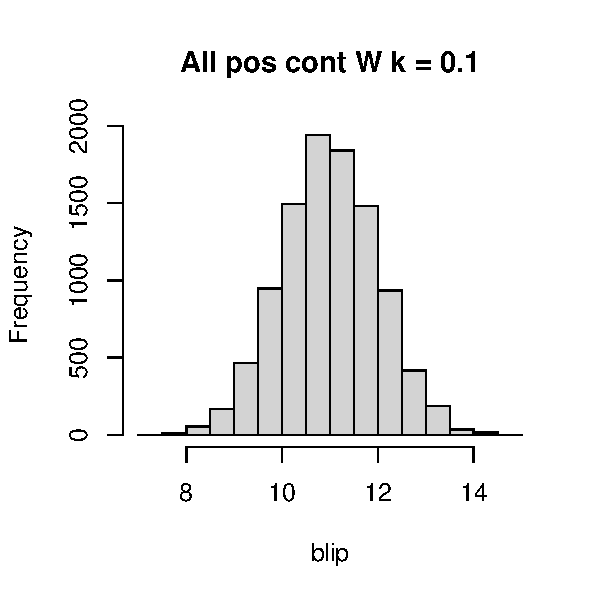
\includegraphics[width=\maxwidth]{figure/unnamed-chunk-4-7} 
\begin{kframe}\begin{verbatim}
##                     desc    bias_psi bias_cont_EY0 bias_cont_EY1     var_psi
## 1 All pos cont W k = 0.1 -0.01046928  -0.003207263  -0.003207263 0.003586811
##   var_cont_EY0 var_cont_EY1 cov_psi cov_cont_EY0 cov_cont_EY1 cov_da_psi
## 1  0.000463368  0.004381832   0.929        0.934        0.954      0.988
##   cov_da_cont_EY0 cov_da_cont_EY1 regret tauP0vtauPn
## 1           0.948           0.976      0 0.004620943
\end{verbatim}
\end{kframe}
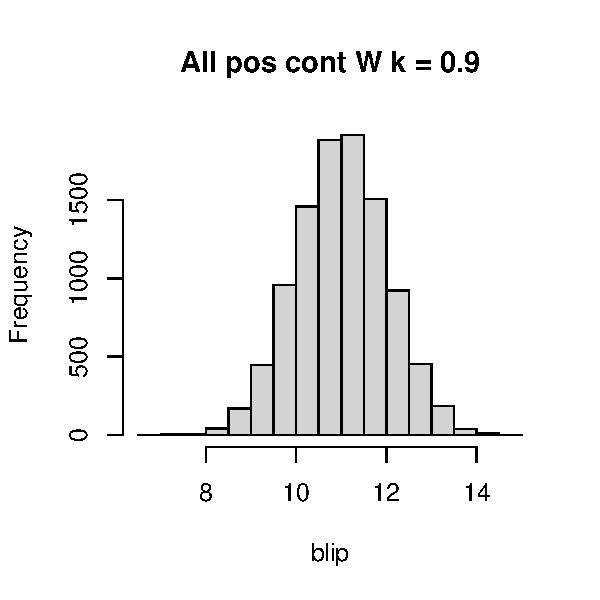
\includegraphics[width=\maxwidth]{figure/unnamed-chunk-4-8} 
\begin{kframe}\begin{verbatim}
##                     desc    bias_psi bias_cont_EY0 bias_cont_EY1     var_psi
## 1 All pos cont W k = 0.9 0.003405452   -0.00432496   -0.00432496 0.005915347
##   var_cont_EY0 var_cont_EY1 cov_psi cov_cont_EY0 cov_cont_EY1 cov_da_psi
## 1  0.004566665 0.0004098842   0.941        0.937        0.896      0.996
##   cov_da_cont_EY0 cov_da_cont_EY1 regret  tauP0vtauPn
## 1           0.969           0.964      0 -0.001170377
\end{verbatim}
\end{kframe}
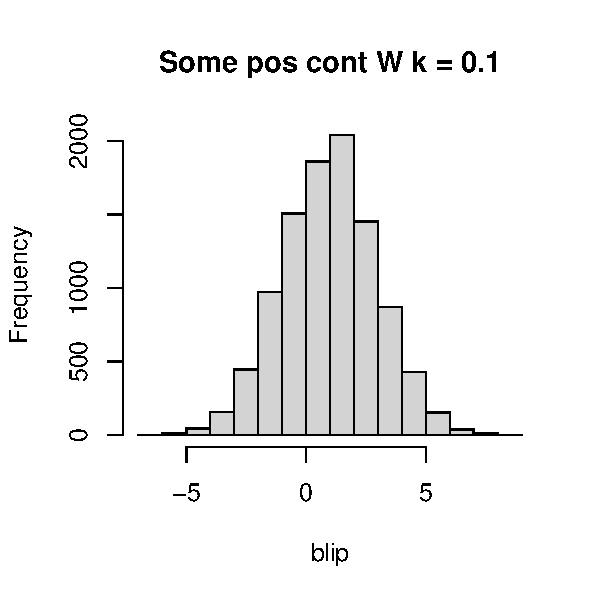
\includegraphics[width=\maxwidth]{figure/unnamed-chunk-4-9} 
\begin{kframe}\begin{verbatim}
##                      desc     bias_psi bias_cont_EY0 bias_cont_EY1    var_psi
## 1 Some pos cont W k = 0.1 -0.003840838   0.004360377   0.004360377 0.00299759
##   var_cont_EY0 var_cont_EY1 cov_psi cov_cont_EY0 cov_cont_EY1 cov_da_psi
## 1 0.0005600421  0.007404762   0.945        0.953        0.938      0.978
##   cov_da_cont_EY0 cov_da_cont_EY1 regret  tauP0vtauPn
## 1           0.974            0.99      0 -0.001144055
\end{verbatim}
\end{kframe}
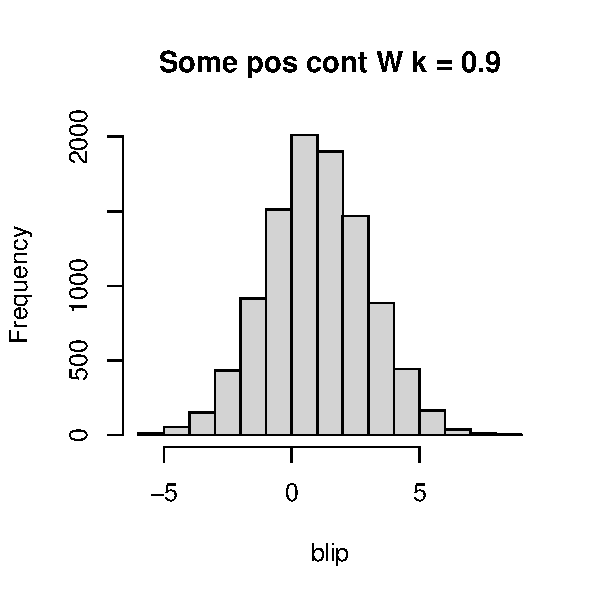
\includegraphics[width=\maxwidth]{figure/unnamed-chunk-4-10} 
\begin{kframe}\begin{verbatim}
##                      desc    bias_psi bias_cont_EY0 bias_cont_EY1     var_psi
## 1 Some pos cont W k = 0.9 0.001392494   0.005327546   0.005327546 0.002407114
##   var_cont_EY0 var_cont_EY1 cov_psi cov_cont_EY0 cov_cont_EY1 cov_da_psi
## 1  0.005180188  0.001924184   0.941        0.942        0.944      0.968
##   cov_da_cont_EY0 cov_da_cont_EY1        regret tauP0vtauPn
## 1           0.995           0.986 -0.0004422375           0
\end{verbatim}
\end{kframe}
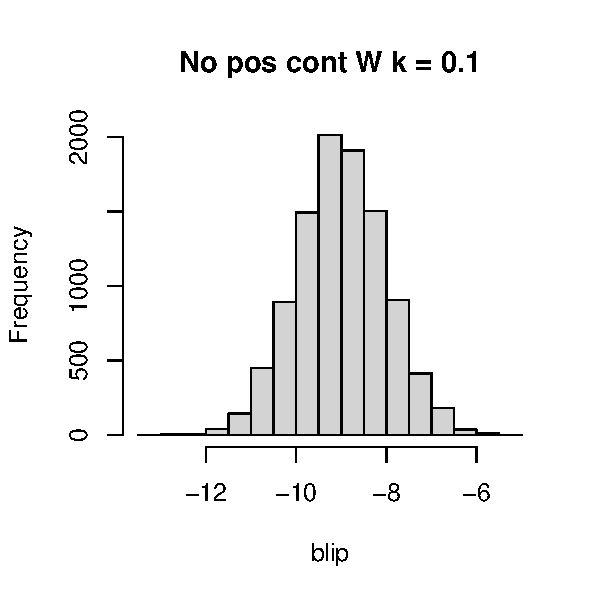
\includegraphics[width=\maxwidth]{figure/unnamed-chunk-4-11} 
\begin{kframe}\begin{verbatim}
##                    desc    bias_psi bias_cont_EY0 bias_cont_EY1    var_psi
## 1 No pos cont W k = 0.1 0.004423212    0.00855373    0.00855373 0.00297045
##   var_cont_EY0 var_cont_EY1 cov_psi cov_cont_EY0 cov_cont_EY1 cov_da_psi
## 1 1.300241e-33   0.00504797   0.951            0        0.946      0.984
##   cov_da_cont_EY0 cov_da_cont_EY1 regret tauP0vtauPn
## 1            0.95           0.973      0           0
\end{verbatim}
\end{kframe}
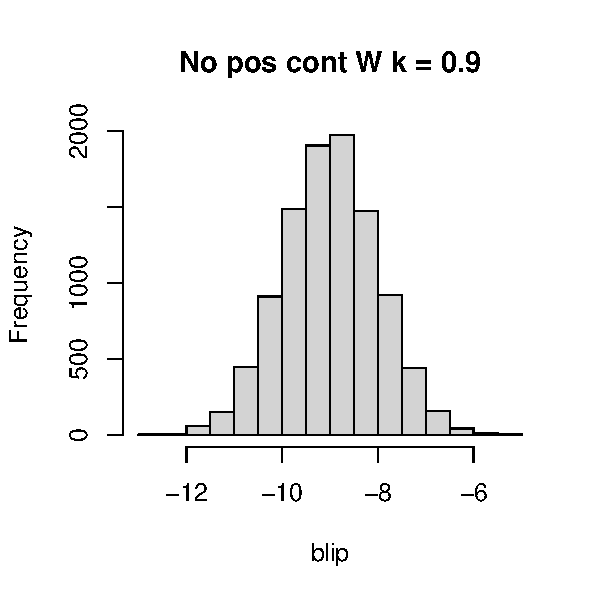
\includegraphics[width=\maxwidth]{figure/unnamed-chunk-4-12} 
\begin{kframe}\begin{verbatim}
##                    desc     bias_psi bias_cont_EY0 bias_cont_EY1    var_psi
## 1 No pos cont W k = 0.9 -0.003828655  -0.004742516  -0.004742516 0.00297045
##   var_cont_EY0 var_cont_EY1 cov_psi cov_cont_EY0 cov_cont_EY1 cov_da_psi
## 1 1.300241e-33   0.00504797   0.954            0        0.942      0.984
##   cov_da_cont_EY0 cov_da_cont_EY1 regret tauP0vtauPn
## 1            0.95           0.973      0           0
\end{verbatim}
\end{kframe}
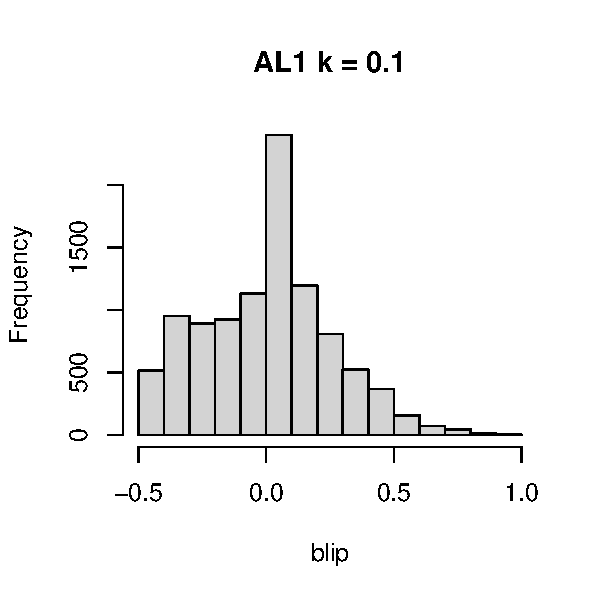
\includegraphics[width=\maxwidth]{figure/unnamed-chunk-4-13} 
\begin{kframe}\begin{verbatim}
##          desc    bias_psi bias_cont_EY0 bias_cont_EY1      var_psi var_cont_EY0
## 1 AL1 k = 0.1 -0.01802401   -0.01981226   -0.01981226 0.0005120323 0.0001434307
##   var_cont_EY1 cov_psi cov_cont_EY0 cov_cont_EY1 cov_da_psi cov_da_cont_EY0
## 1 0.0009067548   0.878        0.497        0.902      0.965           0.926
##   cov_da_cont_EY1      regret tauP0vtauPn
## 1           0.961 -0.01730605   0.1200004
\end{verbatim}
\end{kframe}
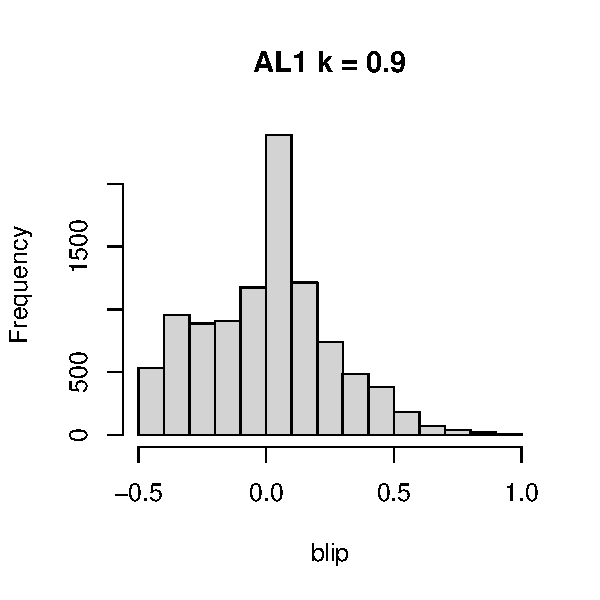
\includegraphics[width=\maxwidth]{figure/unnamed-chunk-4-14} 
\begin{kframe}\begin{verbatim}
##          desc    bias_psi bias_cont_EY0 bias_cont_EY1      var_psi var_cont_EY0
## 1 AL1 k = 0.9 -0.03105257   -0.03167082   -0.03167082 0.0007370152  0.000722881
##   var_cont_EY1 cov_psi cov_cont_EY0 cov_cont_EY1 cov_da_psi cov_da_cont_EY0
## 1 0.0007460663    0.68        0.656        0.694      0.943           0.948
##   cov_da_cont_EY1      regret   tauP0vtauPn
## 1           0.928 -0.02706894 -4.341017e-06
\end{verbatim}
\end{kframe}
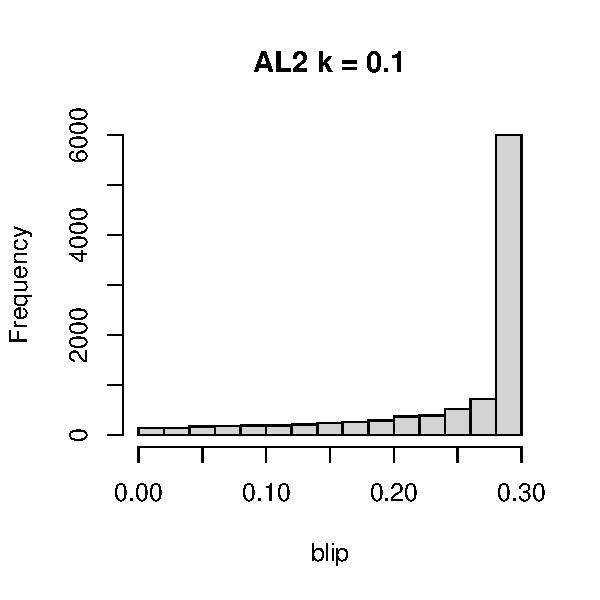
\includegraphics[width=\maxwidth]{figure/unnamed-chunk-4-15} 
\begin{kframe}\begin{verbatim}
##          desc      bias_psi bias_cont_EY0 bias_cont_EY1      var_psi
## 1 AL2 k = 0.1 -0.0001949351  0.0008555856  0.0008555856 0.0004238784
##   var_cont_EY0 var_cont_EY1 cov_psi cov_cont_EY0 cov_cont_EY1 cov_da_psi
## 1 9.876248e-05  0.000845078   0.943        0.932        0.943      0.945
##   cov_da_cont_EY0 cov_da_cont_EY1       regret  tauP0vtauPn
## 1           0.943           0.947 -0.001463191 -0.006965769
\end{verbatim}
\end{kframe}
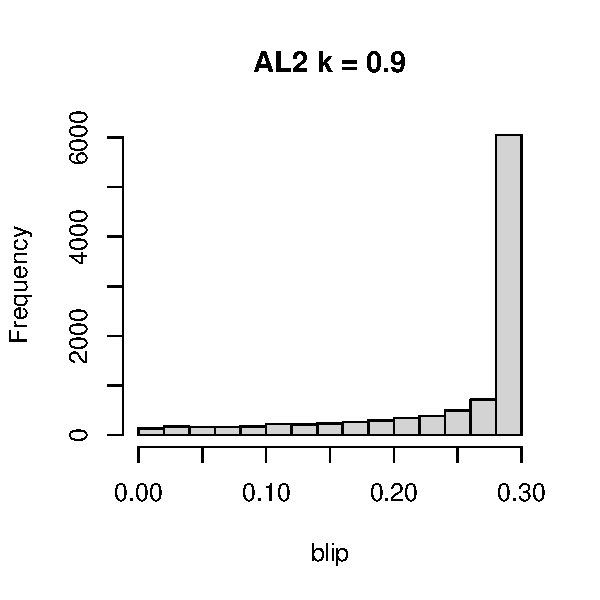
\includegraphics[width=\maxwidth]{figure/unnamed-chunk-4-16} 
\begin{kframe}\begin{verbatim}
##          desc      bias_psi bias_cont_EY0 bias_cont_EY1      var_psi
## 1 AL2 k = 0.9 -0.0005044598  -0.002503939  -0.002503939 0.0005255853
##   var_cont_EY0 var_cont_EY1 cov_psi cov_cont_EY0 cov_cont_EY1 cov_da_psi
## 1 0.0008731405 0.0001151983   0.939        0.942        0.919      0.946
##   cov_da_cont_EY0 cov_da_cont_EY1       regret tauP0vtauPn
## 1           0.946           0.945 -0.002353075  -0.0278073
\end{verbatim}
\end{kframe}
\end{knitrout}







\end{document}
